\documentclass[11pt]{beamer}
\usetheme{Boadilla}
\usepackage[utf8]{inputenc}
\usepackage[francais]{babel}
\usepackage[T1]{fontenc}
\usepackage{amsmath}
\usepackage{amsfonts}
\usepackage{amssymb}
\usepackage{graphicx}
\usepackage{tikz}

\def\CS{\text{CS}}
\def\gint{\displaystyle\int}
\def\gsum{\displaystyle\sum\limits}
\def\dxi{\tilde{\delta}^H_{\xi}}
\def\deta{\tilde{\delta}^H_{\eta}}
\def\fxi{\tilde{\mathcal{F}}_{\xi}}
\def\feta{\tilde{\mathcal{F}}_{\eta}}
\def\Vect{\text{Vect}}

\author[M. Brachet]{Matthieu Brachet}
\title[Soutenance de thèse]{Schémas compacts hermitiens sur la Sphère - Applications en climatologie et océanographie numérique}
%\setbeamercovered{transparent} 
%\setbeamertemplate{navigation symbols}{} 
%\logo{} 
%\institute{} 
\date[3-7-2018]{Mardi 3 Juillet 2018} 
%\subject{} 
\begin{document}

\begin{frame}
\titlepage
\begin{flushright}
\includegraphics[scale=.21]{ul.png}
\includegraphics[scale=.25]{iecl.jpg}
\end{flushright}
\end{frame}

%% ***************************************************************

\begin{frame}
\tableofcontents
\end{frame}

%% ***************************************************************
\section{Introduction}
\begin{frame}{Introduction}
\begin{block}{Enjeux}
Prévisions de la dynamique atmosphérique.
\end{block}

\begin{alertblock}{}
Problème difficile :
\begin{itemize}
\item Equations complexes,
\item Contexte sphérique,
\item Nombreuses échelles à prendre en compte.
\end{itemize}
\end{alertblock}

\begin{exampleblock}{Objectif :}
\begin{itemize}
\item Conception d'un schéma numérique pour un modèle simplifié : les équations \textbf{Shallow Water sphériques}.
\end{itemize}
\end{exampleblock}
\end{frame}



\begin{frame}{}
\begin{block}{Analyse numérique :}
\begin{itemize}
\item Conception et étude d'un schéma innovant.
\item Schémas centrés en espace pour des équations hyperboliques.
\end{itemize}
\end{block}

\begin{block}{Code de calcul :}
\begin{itemize}
\item Code en Matlab.
\item Séquentiel, pas de calculs sur GPU.
\item Sur une station de travail (Intel XEON CPU E5620 v2 - 2.40GHz, 47.1 Gio).
\end{itemize}
\end{block}
\end{frame}







\begin{frame}{Grille Yin-Yang}
\begin{columns}
\column{0.45\textwidth}
\begin{center}
\includegraphics[scale=.5]{yinyang.png}
\end{center}

\column{0.45\textwidth}
Combinaison de \textbf{deux grilles Longitude-Latitude} tronquées.

\begin{itemize}
\item Volumes finis : Li \textit{et al.}, 2008.
\item Éléments finis de Galerkin discontinu : Hall \textit{et al.}, 2013.
\end{itemize}
\end{columns}
\end{frame}



\begin{frame}{Grille Icosaèdrale}
\begin{columns}
\column{0.45\textwidth}
\begin{center}
\includegraphics[scale=.45]{ico.png}
\end{center}

\column{0.45\textwidth}
Maillage d'un \textbf{icosaèdre} projeté sur la sphère.

\begin{itemize}
\item Volumes finis : Thuburn \textit{et al.}, 2014.
\item Éléments finis de Galerkin discontinu : Giraldo \textit{et al.}, 2002.
\end{itemize}
\end{columns}
\end{frame}



\begin{frame}{Cubed-Sphere}
\begin{columns}
\column{0.45\textwidth}
\begin{center}
\includegraphics[scale=.2]{cs.png}
\end{center}

\column{0.45\textwidth}

Maillage d'un \textbf{cube} projeté sur la Sphère.

\begin{itemize}
\item Volumes finis : Ullrichn \textit{et al.}, 2010.

\item \'Eléments finis de Galerkin : Nair \textit{et al.}, 2005.
\end{itemize}


\end{columns}
\end{frame}

%% ***************************************************************

\section{La Cubed-Sphere}
\begin{frame}{Panels}
\begin{columns}
\column{0.45\textwidth}
\begin{figure}[htbp]
\begin{center}
\includegraphics[scale=0.2]{panelI.jpg}
\end{center}
\end{figure}

\column{0.45\textwidth}
\begin{itemize}
\item $C_{II}^1 = \Vect(\mathbf{i}+\mathbf{k}, \mathbf{j}) \cap \mathbb{S}_a^2$,
\item le cercle $C_{II}^2$ est une rotation de $C_{II}^1$ d'un angle de $\pi/2$ autour de $(Oy)$,
\item $C_V^1 = \Vect(\mathbf{i}-\mathbf{j}, \mathbf{k}) \cap \mathbb{S}_a^2$,
\item $C_V^2$ est une rotation de $C_V^1$ d'un angle de $\pi/2$ autour de $(Oz)$.
\end{itemize}

\begin{block}{}
Les grands cercles $C_{II}^1$, $C_{II}^2$, $C_V^1$ et $C_V^1$ délimitent le panel $(I)$.
\end{block}
\end{columns}
\end{frame}









\begin{frame}{La grille Cubed-Sphere}
\begin{columns}
\column{0.45\textwidth}
\begin{figure}[htbp]
\begin{center}
\includegraphics[scale=.27]{cs_cercles.png}
\end{center}
\caption{Le panel $(I)$ est constitué des points d'intersections d'un ensemble de grands cercles.}
\end{figure}  

\column{0.5\textwidth}
\begin{itemize}
\item 2 ensembles de grands cercles $C_i^{(1)}$ et $C_j^{(2)}$, $-N/2 \leq i,j \leq N/2$,

\item $C_0^{(1)}$ et $C_0^{(2)}$ s'intersectent avec un angle de $90$ degrés

\item Les points $\mathbf{x}_{i,j}=C_i^{(1)} \cap C_j^{(2)}$ sont les points de maillage sur un panel de la Cubed-Sphere.
\end{itemize}

\begin{block}{}
On reproduit 6 fois le processus pour couvrir la sphère $\mathbb{S}_a^2$.
\end{block}

\end{columns}
\end{frame}













\begin{frame}{La grille Cubed-Sphere: 6 panels}
\begin{figure}
\begin{center}
\hspace{-1.cm}
\includegraphics[scale=0.28]{plot_CS.png}
\caption{La Cubed-Sphere avec $N=16$ ($16^2$ cellules par panels).
}
\end{center}
\end{figure}
\end{frame}










\begin{frame}{Localisation d'un point sur un panel}
\begin{columns}
\column{0.45\textwidth}
\begin{figure}[htbp]
\begin{center}
\includegraphics[scale=.27]{cs_angles.png}
\end{center}
\caption{Sur un panel, un point $\mathbf{x}$ est localisé par $\xi$ et $\eta$.}
\end{figure}
\column{0.5\textwidth}
\begin{itemize}
\item $(\xi_i, \eta_j)$ avec $-N/2 \leq i,j \leq N/2$ forment un maillage régulier sur un panel.
\item Le pas de discrétisation est
$$
\Delta \xi = \Delta \eta = \dfrac{\pi}{2N}.
$$ 
\end{itemize}
\end{columns}
\end{frame}











\begin{frame}{}
\begin{columns}
\column{0.45\textwidth}
\begin{figure}[htbp]
\begin{center}
\includegraphics[scale=.27]{cs_angles.png}
\end{center}
\caption{Sur un panel, un point $\mathbf{x}$ est localisé par $\xi$ et $\eta$.}
\end{figure}
\column{0.5\textwidth}
\begin{itemize}
\item Une base en $\mathbf{x}$ est $$(\mathbf{g}_{\xi}, \mathbf{g}_{\eta}) = (\partial_{\xi} \mathbf{x}, \partial_{\eta} \mathbf{x}).$$

\item Le tenseur métrique en $\mathbf{x} \in \mathbb{S}_R^2$ est
\begin{equation*}
G=\begin{bmatrix}
\mathbf{g}_{\xi} \cdot \mathbf{g}_{\xi} & \mathbf{g}_{\xi} \cdot \mathbf{g}_{\eta} \\
\mathbf{g}_{\eta} \cdot \mathbf{g}_{\xi} & \mathbf{g}_{\eta} \cdot \mathbf{g}_{\eta} 
\end{bmatrix}
\end{equation*}

\item La base duale en $\mathbf{x} \in \mathbb{S}^2_a $ est $(\mathbf{g}^\xi(\mathbf{x}),\mathbf{g}^\eta(\mathbf{x}))$ donnée par
$$
\begin{bmatrix}
\mathbf{g}^{\xi} \\ \mathbf{g}^{\eta} 
\end{bmatrix}
=
\mathbf{G}^{-1} \cdot
\begin{bmatrix}
\mathbf{g}_{\xi} \\ \mathbf{g}_{\eta} 
\end{bmatrix}.
$$
\end{itemize}
\end{columns}
\end{frame}













\begin{frame}{Bilan}
\begin{itemize}
\item La Cubed-Sphere est déduite de 6 réseaux de $N+1$ grands cercles chacun.

\item Elle est composée de $6N^2+2$ points :
\begin{itemize}
\item $8$ coins de la Cubed-Sphere,
\item $12(N-1)$ points appartenant à deux panels exactement,
\item $6(N-1)^2$ points intérieurs des panels.
\end{itemize}

\item On pose $\Delta \xi = \Delta \eta = \dfrac{\pi}{2N}$ le pas de discrétisation.
\end{itemize}
\end{frame}















\begin{frame}{Produit scalaire sur la Cubed-Sphere}

On pose $\bar{\mathbf{G}}_{i,j} = \det ( \mathbf{G}(\mathbf{x}_{i,j}^{(k)}))$.

\begin{block}{}
Soient $\mathfrak{u}$ et $\mathfrak{v}$ deux fonctions de grilles sur la Cubed-Sphere. On définit
$$<\mathfrak{u},\mathfrak{v}>_{\CS} = \gsum_{(k) = (I)}^{(VI)} \gsum_{-N/2 \leq i,j \leq N/2} \omega_{i,j} \sqrt{\bar{\mathbf{G}}_{i,j}} \mathfrak{u}_{i,j}^{(k)} \bar{\mathfrak{v}}_{i,j}^{(k)}$$
alors $<\cdot, \cdot>_{\CS}$ est un \textbf{produit scalaire} si les coefficients $\omega_{i,j}$ sont positifs.
\end{block}
\end{frame}




\begin{frame}
Soient $m, m' \in \mathbb{Z}$, $l \leq |m|$ et $l' \leq |m'|$, alors pour $\mathbf{Y}_m^l$ et $\mathbf{Y}_{m'}^{l'}$ des harmoniques sphériques, on a 
$$
<\mathbf{Y}_m^l, \mathbf{Y}_{m'}^{l'}>_{L^2} = \delta_{m,m'}\delta_{l,l'}.
$$
Cette propriété est partiellement vérifiée par $<\cdot, \cdot>_{\CS}$ :

\begin{block}{}
Si on a
$$
\omega_{i,j} = \omega_{-i,-j} = \omega_{-i,j} = \omega_{i,-j}>0
$$
pour tous $i$ et $j$. Alors on a
$$
<\mathbf{Y}_m^{l,*}, \mathbf{Y}_{m'}^{l',*}>_{L^2} = 0
$$
lorsque
\begin{itemize}
\item $m+m'$ est impair ou,
\item $l+l'$ est impair.
\end{itemize}
\end{block}
\end{frame}








\begin{frame}{}
\begin{block}{Maillage Cubed-Sphere}
\begin{itemize}
\item Construction d'un maillage couvrant la sphère.
\item Pas de discrétisation régulier.
\item Géométrie par panel quasi-cartésienne.
\end{itemize}
\end{block}

\begin{block}{Produit scalaire discret}
\begin{itemize}
\item Construction d'un produit scalaire discret.
\item Très bonnes propriétés d'orthogonalité des harmoniques sphériques.
\end{itemize}
\end{block}
\end{frame}






%% ***************************************************************
\section{Opérateurs discrets sur la Cubed-Sphere}
\begin{frame}{Opérateurs discrets sur la Cubed-Sphere}
Les opérateurs sont définis en coordonnées $(\xi,\eta)$ par
\begin{block}{}
\begin{itemize}
\item \textbf{Gradient :}
$$
\nabla_T h = \mathbf{g}^{\xi} \dfrac{\partial h}{\partial \xi} + \mathbf{g}^{\eta} \dfrac{\partial h}{\partial \eta},
$$
\item \textbf{Divergence :}
$$
\nabla_T \cdot \mathbf{u} = \mathbf{g}^{\xi} \cdot \dfrac{\partial \mathbf{u}}{\partial \xi} + \mathbf{g}^{\eta} \cdot \dfrac{\partial \mathbf{u}}{\partial \eta},
$$
\item \textbf{Vorticité :}
$$
\text{vort}(\mathbf{u}) = \left( \mathbf{g}^{\xi} \wedge \dfrac{\partial \mathbf{u}}{\partial \xi} + \mathbf{g}^{\eta} \wedge \dfrac{\partial \mathbf{u}}{\partial \eta} \right) \cdot \mathbf{n}.
$$
\end{itemize}
\end{block}
Il s'agit d'approcher $\dfrac{\partial}{\partial \xi}$ et $\dfrac{\partial}{\partial \eta}$ sur les points de la Cubed-Sphere.
\end{frame}





\begin{frame}
\begin{columns}
\column{0.5\textwidth}
\begin{figure}
\begin{center}
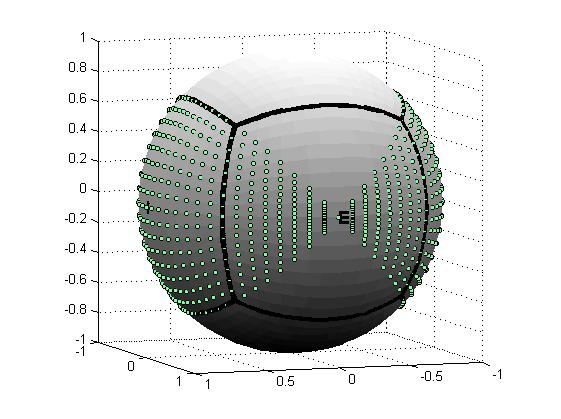
\includegraphics[scale=.3]{fig22.jpg}
\end{center}
\end{figure}

\column{0.5\textwidth}
\begin{block}{}
\begin{itemize}
\item Si les données sont disponible sur un grand cercle complet : utilisation de schéma aux différences finies pour le calcul de $\partial_{\xi}$ et $\partial_{\eta}$.

\item Système de coordonnées régulier.

\item Périodicité sur les grands cercles.
\end{itemize}

\end{block}



\end{columns}
\end{frame}














\begin{frame}{Discrétisation sur un grand cercle}
On se donne $(\mathfrak{u}_j)_{j\in \mathbb{Z}}$ une fonction de grille périodique
\begin{figure}[htbp]
\begin{center}
\begin{tikzpicture}[scale=1]
	\draw [>=stealth, <->] (-2,0.2) -- (-1,.2) ;
	\draw (-1.5,.3) node[above] {$\Delta \xi$} ;
	\draw [>=stealth, <->] (-3,0) -- (3,0) ;
	\draw (-2,0) node {$\bullet$} ;
	\draw (-2,-.2) node[below] {$\cdots$} ;
	\draw (-1,0) node {$\bullet$} ;
	\draw (-1,-.2) node[below] {$\mathfrak{u}_{j-1}$} ;
	\draw (0,0) node {$\bullet$} ;
	\draw (0,-.2) node[below] {$\mathfrak{u}_j$} ;
	\draw (1,0) node {$\bullet$} ;
	\draw (1,-.2) node[below] {$\mathfrak{u}_{j+1}$} ;
	\draw (2,0) node {$\bullet$} ;
	\draw (2,-.2) node[below] {$\cdots$} ;
\end{tikzpicture}
\end{center}
\end{figure}

\begin{block}{Formule locale d'ordre 2 :}
L'opérateur $\delta_{\xi}$ défini par
$$
\dfrac{\mathfrak{u}_{j+1}-\mathfrak{u}_{j-1}}{2 \Delta \xi} = \delta_{\xi} \mathfrak{u}_j \text{ avec } j \in \mathbb{Z},
$$
permet une approximation de la dérivée première :
$$
\delta_{\xi} u^*_j = \partial_{\xi} u_j + \mathcal{O} \left( \Delta \xi^2 \right)
$$
avec $u \in \mathcal{C}^3$.
\end{block}
\end{frame}






\begin{frame}{}
\begin{block}{Opérateur hermitien $\delta_{\xi}^H$ :}
L'opérateur de \textbf{dérivation hermitien} est définit par
$$
\delta_{\xi}^H = \sigma_{\xi}^{-1} \circ \delta_{\xi}
$$
où $\sigma_{\xi}$ et $\delta_{\xi}$ sont définis par
$$
\underbrace{\dfrac{1}{6}\mathfrak{u}_{\xi,j-1} + \dfrac{4}{6}\mathfrak{u}_{\xi,j} + \dfrac{1}{6} \mathfrak{u}_{\xi,j+1} }_{\sigma_{\xi} \mathfrak{u}_{\xi,j}} \text{ et } \underbrace{\dfrac{\mathfrak{u}_{j+1}-\mathfrak{u}_{j-1}}{2 \Delta \xi}}_{\delta_{\xi} \mathfrak{u}_j}.
$$
\end{block}

\begin{block}{Approximation d'ordre 4 :}
Approximation de la dérivée première à l'ordre 4:
$$
\delta_{\xi}^H u^*_j = \partial_{\xi} u_j + \mathcal{O} \left( \Delta \xi^4 \right)
$$
avec $u \in \mathcal{C}^5$.
\end{block}
\end{frame}










\begin{frame}
\begin{columns}
\column{0.45\textwidth}
\textbf{Calcul de $\dxi$ :}
\begin{enumerate}
\item Complétion des données sur un grand cercle complet par \textbf{spline cubique},
\item Calcul de la dérivée approchée en utilisant $\delta_{\xi}^H$.
\end{enumerate}
On procède de même pour le calcul de $\deta$.

\column{0.5\textwidth}
\begin{center}
\includegraphics[scale=.28]{CS_interp.png}
\end{center}
\end{columns}

$\Rightarrow$ On remplace $\dfrac{\partial}{\partial \xi}$ et $\dfrac{\partial}{\partial \eta}$ par $\dxi$ et $\deta$ calculés sur la Cubed-Sphere.
\end{frame}


















\begin{frame}{Opérateurs discrets sur la Cubed-Sphere}
Les opérateurs discrets sont définis par
\begin{block}{}
\begin{itemize}
\item \textbf{Gradient discret:}
$$
\nabla_{T,\Delta} \mathfrak{h} = \mathbf{g}^{\xi} \dxi \mathfrak{h} + \mathbf{g}^{\eta} \deta \mathfrak{h},
$$
\item \textbf{Divergence discrète :}
$$
\nabla_{T,\Delta} \cdot \mathfrak{u} = \mathbf{g}^{\xi} \cdot \dxi \mathfrak{u} + \mathbf{g}^{\eta} \cdot \deta \mathfrak{u},
$$
\item \textbf{Vorticité discrète :}
$$
\text{vort}_{\Delta} (\mathfrak{u}) = \left( \mathbf{g}^{\xi} \wedge \dxi \mathfrak{u} + \mathbf{g}^{\eta} \wedge \deta \mathfrak{u} \right) \cdot \mathbf{n}.
$$
\end{itemize}
\end{block}
\end{frame}




\begin{frame}{Consistance des opérateurs discrets}
Soit $h$ une fonction scalaire sur $\mathbb{S}_a^2$ et $\mathbf{u}$ un champ vectoriel sur $\mathbb{S}_a^2$. Si $h$ et $\mathbf{u}$ sont réguliers, alors on a :
\begin{block}{}
\begin{itemize}
\item \textbf{Consistance du gradient :}
$$
(\nabla_T h)^* - \nabla_{T,\Delta} h^* = \mathcal{O}(\Delta \xi^3),
$$
\item \textbf{Consistance de la divergence :}
$$
(\nabla_T \cdot \mathbf{u})^* - \nabla_{T,\Delta} \cdot \mathbf{u}^* = \mathcal{O}(\Delta \xi^3),
$$
\item \textbf{Consistance de la vorticité :}
$$
\text{vort}(\mathbf{u})^* - \text{vort}_{\Delta}(\mathbf{u}^*) = \mathcal{O}(\Delta^3).
$$
\end{itemize}
\end{block}

\begin{alertblock}{}
\textbf{Ordre 4} observé dans les expériences numériques.
\end{alertblock}
\end{frame}








\begin{frame}{Opérateur de filtrage}

En suivant le même procédé on construit les opérateurs de filtrage $\fxi$ et $\feta$. On définit alors :
$$
\mathcal{F} = \dfrac{1}{2} \left( \fxi \circ \feta + \feta \circ \fxi \right),
$$

\begin{block}{}
Si $h$ est une fonction régulière sur la sphère, on a:
$$
\mathcal{F}(h^*) - h^* = \mathcal{O} \left( \Delta \xi^4 \right).
$$
\end{block}
\end{frame}









\begin{frame}{Opérateurs discrets}
\begin{block}{}
\begin{itemize}
\item Construction d'opérateurs différentiels discrets et hermitiens sur la Cubed-Sphere.
\item Ordre 3 démontré, ordre 4 observé.
\end{itemize}
\end{block}

\begin{block}{}
\begin{itemize}
\item Construction systématique des opérateurs.
\item Très facile de remplacer $\delta_{\xi}^H$ par un autre opérateur. 
\end{itemize}
\end{block}

\begin{alertblock}{}
Les splines cubiques limites la montée en ordre.
\end{alertblock}

\end{frame}










%% *****************************************************************
\section{Cas de la dimension 1}
\begin{frame}{Equation de transport 1D}
Dans le cadre périodique, on considère l'équation :
$$
\left\lbrace
\begin{array}{rcl}
\dfrac{\partial u}{\partial t} + c \dfrac{\partial u}{\partial x} & = & 0 \\
u(t=0,x) & = & u_0(x)
\end{array}
\right. \text{ pour } x \in [0,L] \text{ et } t>0.
$$
\begin{block}{}
\textbf{Première étape : discrétisation en espace.}
\end{block}
Equation semi-discrétisée :
$$
\left\lbrace
\begin{array}{rcl}
\dfrac{\partial \mathfrak{u}}{\partial t} + c \delta_x^H \mathfrak{u} & = & 0 \\
\mathfrak{u}(t=0) & = & u_0^*
\end{array}
\right. \text{ pour } x \in [0,L] \text{ et } t>0.
$$
\end{frame}


\begin{frame}{}
\begin{block}{Proposition}
Si $u$ est régulière, alors on a
$$
\| \mathfrak{u}(t) - u(t,\cdot)^* \|_{h,\text{pér}} \leq C t \Delta \xi^4 \| \partial_{\xi}^{(5)}u \|_{\infty}
$$
avec $C>0$ indépendant de $t$, $\Delta \xi$ et $u$.
\end{block}

\begin{block}{Discrétisation en temps :}
Méthode de Runge-Kutta d'ordre 4 avec étape de filtrage.
\end{block}
\end{frame}


\begin{frame}{Schéma de référence}
\begin{block}{Runge-Kutta d'ordre 4 + Filtre spatial
}
\begin{enumerate}
\item $K^{(1)} = - c \delta_{\xi}^H \mathfrak{u}^n$,
\item $K^{(2)} = - c \delta_{\xi}^H \left( \mathfrak{u}^n + \dfrac{\Delta t}{2} K^{(1)} \right)$,
\item $K^{(3)} = - c \delta_{\xi}^H \left( \mathfrak{u}^n + \dfrac{\Delta t}{2} K^{(2)} \right)$,
\item $K^{(4)} = - c \delta_{\xi}^H \left( \mathfrak{u}^n + \Delta t K^{(3)} \right)$
\item $\hat{\mathfrak{u}}^{n+1} = \mathfrak{u}^n + \frac{\Delta t}{6} \left( K^{(1)} + 2 K^{(2)} + 2 K^{(3)} + K^{(4)} \right)$
\item $\mathfrak{u}^{n+1} = \mathcal{F}(\hat{\mathfrak{u}}^{n+1})$
\end{enumerate}
\end{block}
\end{frame}


\begin{frame}{Opérateur de filtrage}
L'opérateur de filtrage est donné par
$$
\mathcal{F} (\mathfrak{u})_j = \gsum_{i=-5}^5 f_i \mathfrak{u}_{i+j} 
$$
\begin{columns}
\column{0.45\textwidth}
Les coefficients sont donnés par
$$
\begin{bmatrix}
f_0\\
f_1 = f_{-1}\\
f_2 = f_{-2}\\
f_3 = f_{-3}\\
f_4 = f_{-4}\\
f_5 = f_{-5}\\
\end{bmatrix} =
\begin{bmatrix}
772/1024\\
420/1024\\
-240/1024\\
90/1024\\
-20/1024\\
2/1024\\
\end{bmatrix}
$$


\column{0.45\textwidth}
\begin{block}{}
$$
\mathcal{F}(\mathfrak{u}^*)_j = u(x_j) + \mathcal{O} \left( \Delta \xi^{10} \right).
$$
\end{block}

\begin{block}{}
Permet d'atténuer les hautes fréquences et les ondes parasites.
\end{block}
\end{columns}

\end{frame}





\begin{frame}{}
\begin{block}{Proposition}
Le schéma est conservatif au sens où
$$
<\mathfrak{u}^{n+1},\mathfrak{1}>_{\text{pér}} = <\mathfrak{u}^{n},\mathfrak{1}>_{\text{pér}}
$$
pour tout $n \in \mathbb{N}$.
\end{block}


\begin{block}{Proposition}
Le schéma est stable sous la condition
$$
\dfrac{c \Delta t}{\Delta \xi} \leq 2 \sqrt{\dfrac{2}{3}} \leq \lambda_{10}.
$$
Estimation numérique $\lambda_{10} \approx 1.6883$. 
\end{block}
\end{frame}








\begin{frame}{Equation des ondes avec Coriolis constant}
\begin{columns}
\column{0.45\textwidth}
$$
\left\lbrace
\begin{array}{rcl}
\dfrac{\partial \eta}{\partial t} + H \left( \dfrac{\partial u}{\partial x} + \dfrac{\partial v}{\partial y} \right) & = & 0 \\
\dfrac{\partial u}{\partial t} + g \dfrac{\partial \eta}{\partial x} - fv & = & 0\\
\dfrac{\partial v}{\partial t} + g \dfrac{\partial \eta}{\partial y} + fu & = & 0
\end{array}
\right.
$$

Discrétisée par le même procédé.

\column{0.45\textwidth}
\begin{block}{Proposition :}
Ordre 4 en espace et en temps.
\end{block}

\begin{block}{Proposition :}
Conservatif au sens :
$$
<\eta^{n+1},\mathfrak{1}>_{\text{pér}} = <\eta^{n},\mathfrak{1}>_{\text{pér}}
$$
pour tout $n \in \mathbb{N}$.
\end{block}

\begin{block}{Proposition :}
Stable sous la condition
$$
\Delta t \leq \dfrac{2 \sqrt{2}}{\sqrt{\dfrac{6gH}{\Delta \xi^2} + f^2}}.
$$
\end{block}





\end{columns}
\end{frame}

























\begin{frame}{}

\begin{block}{Bilan :}
\begin{itemize}
\item Schéma précis (ordre 4).
\item Bonnes propriétés de stabilité.
\item Schéma conservatif.
\end{itemize}
\end{block}

\begin{exampleblock}{}
Schéma similaire sur la sphère.
\end{exampleblock}

\end{frame}






%% *****************************************************************
\section{Résolution d'équations sur la sphère}
\begin{frame}{Méthode des lignes}
On considère le problème :
$$
\left\lbrace
\begin{array}{rcl}
\dfrac{\partial q}{\partial t} & = & F(q,t) \\
q(t=0,\mathbf{x}) & = & q_0(\mathbf{x})
\end{array}
\right. \text{ avec } \mathbf{x} \in \mathbb{S}_a^2.
$$
\begin{block}{}
\textbf{Première étape : } discrétisation en espace.
\end{block}
$$
\left\lbrace
\begin{array}{rcl}
\dfrac{\partial q}{\partial t} & = & F_{\Delta}(q,t) \\
q(t=0,\mathbf{x}) & = & q_0(\mathbf{x})
\end{array}
\right. \text{ avec } \mathbf{x} \in \mathbb{S}_a^2.
$$
\begin{block}{}
\textbf{Seconde étape : } discrétisation en temps : RK4 avec étape de filtrage.
\end{block}
\end{frame}






\begin{frame}{Schéma de référence}
\begin{block}{Runge-Kutta d'ordre 4 + Filtre spatial
}
\begin{enumerate}
\item $K_1 = F_{\Delta}(\mathfrak{q}^n, t^n)$,
\item $K_2 = F_{\Delta}(\mathfrak{q}^n + \frac{\Delta t}{2} K_1, t^n + \frac{\Delta t}{2})$,
\item $K_3 = F_{\Delta}(\mathfrak{q}^n + \frac{\Delta t}{2} K_2, t^n + \frac{\Delta t}{2})$,
\item $K_4 = F_{\Delta}(\mathfrak{q}^n + \Delta t K_3, t^n + \Delta t)$
\item $\hat{\mathfrak{q}}^{n+1} = \mathfrak{q}^n + \frac{\Delta t}{6} \left( K_1 + 2 K_2 + 2 K_3 + K_4 \right)$
\item $\mathfrak{q}^{n+1} = \mathcal{F}(\hat{\mathfrak{q}}^{n+1})$
\end{enumerate}
\end{block}
\end{frame}









\begin{frame}{Equation d'advection linéaire}

On considère l'équation
$$
\left\lbrace
\begin{array}{rcl}
\dfrac{\partial h}{\partial t} + c(\mathbf{x},t) \cdot \nabla_T h & = & 0  \\
h(t=0,\mathbf{x}) & = & h_0(\mathbf{x})
\end{array}
\right. \text{ avec } \mathbf{x} \in \mathbb{S}_a^2.
$$

\begin{exampleblock}{Test de R. Nair et C. Jablonowski (2008)}
\begin{itemize}
\item Déplacement d'un vortex autour de la sphère,
\item Une solution analytique est disponible $\Rightarrow$ mesure de l'erreur relative.
\end{itemize}
\end{exampleblock}
\end{frame}


\begin{frame}
\begin{figure}
\begin{center}
\includegraphics[height=5cm]{rate_NJ1.png}
\end{center}
\caption{Erreur relative pour l'équation d'advection linéaire. On pose CFL=0.7. Le test est celui de Nair-Jablonowski.}
\end{figure}
\end{frame}

















\begin{frame}{Equation d'advection non linéaire}

On considère l'équation
$$
\left\lbrace
\begin{array}{rcl}
\dfrac{\partial h}{\partial t} + \nabla_T \cdot F(h) & = & 0  \\
h(t=0,\mathbf{x}) & = & h_0(\mathbf{x})
\end{array}
\right. \text{ avec } \mathbf{x} \in \mathbb{S}_1^2.
$$

avec $F(h) = \dfrac{1}{2} h^2 \mathbf{n} \wedge (\mathbf{i} + \mathbf{j} + \mathbf{k})$ 

\begin{exampleblock}{Test de M. Ben-Artzi \text{et al.} (2013)}
\begin{itemize}
\item Conservation de la solution stationnaire 
$$
h_0(x,y,z) = \dfrac{x+y+z}{\sqrt{3}}.
$$
\item La masse doit être conservée.
\end{itemize}
\end{exampleblock}
\end{frame}



\begin{frame}
\begin{figure}[htbp]
\begin{center}
\includegraphics[height=5cm]{rateBA_test3.png}
\end{center}
\caption{Erreur et taux de convergence pour le test stationnaire de l'équation d'advection non linéaire en fonction de $\Delta = a \Delta \xi$. Le pas de temps est donné par $\Delta t = 0.96 \Delta \xi / \pi$. Le temps final est $t=6$.}
\label{fig:benartzi_test3}
\end{figure}
\end{frame}





\begin{frame}
\begin{figure}[htbp]
\begin{center}
\includegraphics[height=4cm]{erreur_test3.png}
\includegraphics[height=4cm]{cons_test3.png}
\end{center}
\caption{ L'erreur en norme et l'erreur de conservation est représentée pour le test stationnaire de l'équation d'advection non linéaire. Le pas de temps est donné par $\Delta t = 0.96 \Delta \xi / \pi$. Le temps final est $t=6$. Le paramètre de la Cubed-Sphere est $N=32$.}
\label{fig:benartzi_test3_hist}
\end{figure}
\end{frame}














%% ****************************************************************************************************************************************

\begin{frame}{Equation Shallow Water}
\begin{block}{}
\begin{equation}
\left\lbrace
\begin{array}{rcl}
\dfrac{\partial h^{\star}}{\partial t} + \nabla_T \cdot \left( h^{\star} \mathbf{v} \right) & = & 0 \\
\dfrac{\partial \mathbf{v}}{\partial t} + \nabla_T \left( \dfrac{1}{2}|\mathbf{v}|^2 + gh \right) + \left( f + \zeta \right) \mathbf{n} \times \mathbf{v} & = & 0
\end{array}
\right.
\end{equation}
où  
\begin{itemize}
\item $h$ est l'épaisseur de fluide et $\mathbf{v}$ le champ de vitesse tangent,
\item $h^{\star}=h-h_s$ avec $h_s$ représentant les reliefs, en général on aura $h_s=0$,
\item $\mathbf{n}$ la normale extérieure, 
\item $\zeta = \left( \nabla_T \times \mathbf{v} \right) \cdot \mathbf{n}$ est la vorticité,
\item $f$ est le paramètre de Coriolis.
\end{itemize}
\end{block}
\end{frame}

%% ***************************************************************************************************************************************

\begin{frame}{Propriétés de conservation}
\begin{block}{}
Si $(h, \mathbf{v})$ est solution des équations Shallow water, les quantités suivantes sont conservées

\begin{itemize}
\item \textbf{masse :} 
$\gint_{\mathbb{S}^2_a} h(t, \mathbf{x}) d \sigma(\mathbf{x})$
\item \textbf{energie :}
$ \gint_{\mathbb{S}^2_a} \left( \dfrac{1}{2}g(h^2 - h_s^2) + \dfrac{1}{2} h | \mathbf{v} |^2 \right) d \sigma(\mathbf{x})$
\item \textbf{enstrophie potentielle :}
$\gint_{\mathbb{S}^2_a} \dfrac{\left( f + \zeta \right)^2}{2gh} d \sigma(\mathbf{x})$
\end{itemize}
\end{block}
\end{frame}

%% ***************************************************************************************************************************************

\begin{frame}{Solution stationnaire pour l'équation Shallow Water [Williamson \textit{et al.}, 1992]}

On a la solution stationnaire suivante :
\begin{exampleblock}{}
\begin{itemize}
\item $h = h_0 - \dfrac{1}{g} \left( a \Omega u_0 + \dfrac{u_0^2}{2} \right)\left( - \cos \lambda \cos \theta \sin \alpha + \sin \theta \cos \alpha \right)^2$
\item $\mathbf{v} = u \mathbf{e}_{\lambda}+ v \mathbf{e}_{\theta}$ avec :
\begin{equation*}
\left\lbrace \begin{array}{rcl}
 u & = & u_0 ( \cos \theta \cos \alpha + \cos \lambda \sin \theta \sin \alpha)\\
 v & = & -u_0 \sin \lambda \sin \alpha
 \end{array} \right.
\end{equation*}
\end{itemize}
\end{exampleblock}

\begin{exampleblock}{}
Pour ce test, on a
$$
f = 2 \Omega (\sin \theta \cos \alpha - \cos \lambda \cos \theta \sin \alpha).
$$
\end{exampleblock}
\end{frame}

%% ***************************************************************************************************************************************

\begin{frame}{SW time independent test case [Williamson and al., 1992]}
\begin{figure}
\includegraphics[height=3cm]{ref_7369088270_snapshot_err_color.png}
\includegraphics[height=3cm]{ref_7369088270_snapshot_intermediaire598.png}
\end{figure}
\begin{itemize}
\item Solution stationnaire avec $\alpha=\pi/4$, la taille de grille est $6 \times 32 \times 32$, le temps final est $T=6$ jours.
\item Erreur relative sur $h$ au temps finale (gauche).
\item $h$ au temps final (droite),
\item $\Delta t \approx 10$ minutes.
\end{itemize}
\end{frame}

%% ***************************************************************************************************************************************

\begin{frame}{Analyse de l'erreur}
\begin{figure}
\includegraphics[height=4cm]{rate_W2_pi4.png}
\end{figure}
\begin{itemize}
\item  On mesure l'erreur relative à $T=6$ jours  :
$$
\dfrac{\| \mathfrak{h}_0 - \mathfrak{h}^n \|}{\| \mathfrak{h}_0 \|}
$$
\item Convergence à l'ordre 4.
\end{itemize}
\end{frame}



\begin{frame}{}
Au temps $t = 5$ jours avec $\alpha = \pi/4$ :
\begin{equation*}
\begin{array}{|c|c|}
\hline
\hline
 & \textbf{Erreur en norme infinie} \\
\hline
 \textbf{Schéma présent :} & 2.75 (-6) \\
 \textbf{VF d'ordre 4 [Chen et al., 2008]} : & 5.86 (-6) \\
 \textbf{VF d'ordre 4 [Ullrich et al., 2011]} : & 1.47 (-6) \\
\hline
\hline
\end{array}
\end{equation*}
pour une grille $6 \times 32 \times 32$ et CFL$=0.9$.

\begin{block}{}
Résultats de précision excellents pour ce test.
\end{block}


\end{frame}


%% ***************************************************************************************************************************************

\begin{frame}{Conservation des quantités}
\begin{figure}
\includegraphics[height=5cm]{ref_7369088270_conservationA.png}
\end{figure}
\begin{itemize}
\item Erreur relative de conservation pour une grille : $6 \times 32 \times 32$ avec $\alpha=\pi/4$ (713 it.).
\item La pire erreur de conservation est de l'ordre de $4 \times 10^{-9}$.
\end{itemize}
\end{frame}





























%% **************************************************************************************************************************************

\begin{frame}{Montagne isolée [Williamson et al., 1992]}

\begin{exampleblock}{}
Test similaire au précédent avec $\alpha = 0$ :

\begin{itemize}
\item $h = h_0 - \dfrac{1}{g} \left( a \Omega u_0 + \dfrac{u_0^2}{2} \right)(\sin \theta)^2$
\item $\mathbf{v} = u_0 \cos \theta \mathbf{e}_{\lambda}$.
\end{itemize}

Cette solution stationnaire est perturbée par une montagne isolée:

$$h_s = h_{s_0} \left( 1 - \dfrac{r}{R} \right)$$

avec $h_{s_0}=2000m$ and $r^2=min(R^2, (\lambda + \pi/2)^2+(\theta - \pi/6)^2)$, $R=\pi/9$.
\end{exampleblock}
\end{frame}

%% ***************************************************************************************************************************************


\begin{frame}{}
\begin{figure}
\includegraphics[height=5cm]{ref_7372184434_snapshot_intermediaire499.png}
\end{figure}
\begin{itemize}
\item $h$ au bout de 5 jours sur une grille $6 \times 32 \times 32$.
\item $\Delta t \approx 10min$.
\end{itemize}
\end{frame}

%% ***************************************************************************************************************************************


\begin{frame}{}
\begin{figure}
\includegraphics[height=5cm]{ref_7372184434_snapshot_intermediaire999.png}
\end{figure}
\begin{itemize}
\item $h$ au bout de 10 jours. La grille est $6 \times 32 \times 32$.
\item $\Delta t \approx 10min$.
\end{itemize}
\end{frame}

%% ***************************************************************************************************************************************


\begin{frame}{}
\begin{figure}
\includegraphics[height=5cm]{ref_7372184434_snapshot_intermediaire1499.png}
\end{figure}
\begin{itemize}
\item $h$ au bout de 15 jours. La grille a pour paramètres : $6 \times 32 \times 32$.
\item $\Delta t \approx 10min$, $2140$ itérations en temps, $6146$ points sur la grille.
\item Les résultats sont très similaires à ceux obtenus par volumes finis ou par Galerkin discontinu d'ordre élevé.
\end{itemize}
\end{frame}

%% ***************************************************************************************************************************************

\begin{frame}{Conservation}
\begin{figure}
\includegraphics[height=4cm]{ref_7368974583_conservationA.jpg}
\end{figure}
\begin{itemize}
\item La grille est $6 \times 32 \times 32$.
\item La masse et l'énergie sont conservées avec une erreur relative proche de $10^{-5}$.
\item L'enstrophie potentielle est conservée avec une erreur relative proche de $10^{-4}$.
\end{itemize}
\end{frame}





\begin{frame}{}
Au temps $t = 15$ jours, erreurs relatives de conservation :
\begin{equation*}
\begin{array}{|c|c|c|}
\hline
\hline
 & \textbf{Energie} & \textbf{Enst. pot.} \\
\hline
 \textbf{Schéma présent avec :} & 1.6 (-5) &-0.9 (-4) \\
 \textbf{VF4 [Chen et al., 2008] (N=32)} : & -4 (-6) & -1.1 (-4) \\
 \textbf{VF4 [Ullrich et al., 2011]} (N=40) : & -3 (-4) & -1.1 (-4) \\
\hline
\hline
\end{array}
\end{equation*}
pour une grille $6 \times 32 \times 32$ et CFL$=0.9$.

\begin{block}{}
Résultats de précision excellents pour ce test.
\end{block}
\end{frame}


























% ***************************************************************************************************************

\begin{frame}{Instabilité Barotrope [J. Galewsky \textit{et al.}, 2004]}

\begin{exampleblock}{}
Une solution stationnaire instable est donnée par
\begin{equation}
\begin{array}{rcl}
\bar{h}(\theta) & = & h_0 + \dfrac{1}{g}\gint^{\theta}_{-\pi/2} a u(\tau) \left[ f + \dfrac{\tan(\tau)}{a} u(\tau) \right] d \tau \\
\mathbf{v}(\lambda,\theta) & = & u(\theta) \mathbf{e}_{\lambda}
\end{array}
\end{equation}
avec :
\begin{itemize}
\item le paramètre de Coriolis $f = 2 \Omega \sin \theta$,
\item $u(\theta)=\left\lbrace
\begin{array}{ll}
\dfrac{u_{max}}{e_n} \exp\left( \dfrac{1}{(\theta-\theta_0)(\theta-\theta_1)} \right) & \text{ if } \theta_0 \leq \theta \leq \theta_1 \\
0 & \text{ else}
\end{array}\right.$\\
 avec $e_n=C^{ste}$, $u_{max} = 80 ms^{-1}$, $\theta_0 = \pi/7$ and $\theta_1 = \pi/2 - \theta_0$.
\end{itemize}
\end{exampleblock}
\end{frame}


%% ***************************************************************************************************************************************

\begin{frame}{}
\begin{exampleblock}{Perturbation}
La fonction précédente est perturbée avec :
\begin{itemize}
\item zonal velocity:
$$\mathbf{v}(\lambda,\theta) = u(\theta) \mathbf{e}_{\lambda}$$
\item perturbation de $h$ par $\bar{h}$:
$$h(\lambda,\theta) = \bar{h}(\lambda,\theta) + \hat{h} \cos \theta \exp \left[ - \left( \dfrac{\lambda}{\alpha} \right)^2 - \left( \dfrac{\theta_2 - \theta}{\beta} \right)^2 \right] \text{, } \hat{h}/\bar{h} \approx 1 \%$$
avec $\theta_2 = \pi/4$, $\alpha = 1/3$ and $\beta = 1/15$.
\end{itemize}
\end{exampleblock}

\begin{block}{}
Ce test est difficile pour la Cubed-Sphere Cubed-Sphere:

\begin{itemize}
\item $h$ varie le long du panel (V)
\item the initial perturbation is located at the boundary between panel (I) and panel (V).
\end{itemize}
\end{block}
\end{frame}

%% ***************************************************************************************************************************************

\begin{frame}{}
\begin{figure}
\includegraphics[height=5cm]{ref_7369437806_snapshot_intermediaire599.jpg}
\end{figure}
\begin{itemize}
\item On représente la vorticité au temps $t=6$jours sur une grille $6 \times 128 \times 128$.
\item Résultats très similaires à ceux obtenus par DG et FV.
\end{itemize}
\end{frame}

%%% ***************************************************************************************************************************************

\begin{frame}{Conservation : masse, énergie et enstrophie potentielle}
\begin{figure}
\includegraphics[height=4cm]{ref_7368306511_massenergy.png}
\includegraphics[height=4cm]{ref_7368306511_enstrophy.png}
\end{figure}
\begin{itemize}
\item Conservation de la masse et de l'énergie (gauche) et de l'enstrophie (droite) sur une grille : $6 \times 128 \times 128$ (Erreur relative). 

\item Propriétés de conservation très satisfaisantes.
\end{itemize}
\end{frame}







\begin{frame}{}
Au temps $t = 6$ jours, erreurs relatives de conservation :
\begin{equation*}
\begin{array}{|c|c|c|}
\hline
\hline
 & \textbf{Energie} & \textbf{Enst. pot.} \\
\hline
 \textbf{Schéma présent avec :} & 1.6 (-5) &-0.9 (-4) \\
 \textbf{VF4 [Chen et al., 2008]} (N=32) : & -4 (-6) & -1.1 (-4) \\
 \textbf{VF4 [Ullrich et al., 2011]} (N=40) : & -3 (-4) & -1.1 (-4) \\
\hline
\hline
\end{array}
\end{equation*}
pour une grille $6 \times 32 \times 32$ et CFL$=0.9$.

\begin{block}{}
Résultats de précision excellents pour ce test.
\end{block}
\end{frame}























\begin{frame}{Test de Rossby-Haurwitz [Williamson et al., 1992]}
\begin{exampleblock}{}
\begin{itemize}
\item Solution analytique pour l'équation de vorticité barotrope.
\item Pas une solution analytique pour Shallow Water.
\item Déplacement d'Ouest en Est.
\item Champ de vitesse initial donné par :
$$
\mathbf{u} = u \mathbf{e}_{\lambda} + v \mathbf{e}_{\theta}
$$
avec 
$$
\left\lbrace
\begin{array}{rcl}
u & = & a \omega \cos \theta + a K \cos^{R-1} \theta \left( R \sin^2 \theta - \cos^2 \theta \right) \cos R \lambda\\
v & = & - a K R \cos^{R-1} \theta \sin \theta \sin R \lambda.
\end{array}
\right.
$$
\item La fonction $h$ est initialement donnée par :
\begin{equation}
gh = gh_0 + a^2 A(\theta) + a^2 B(\theta) \cos R \lambda + a^2 C(\theta) \cos 2 R \lambda,
\end{equation}
avec $A$, $B$ et $C$ des fonctions de $\theta$ analytiques données.
\end{itemize}
\end{exampleblock}
\end{frame}



\begin{frame}{}
\begin{figure}
\includegraphics[height=5cm]{ref_7369145763_snapshot_intermediaire1399.jpg}
\end{figure}
On représente $h$ au temps $t=14$ jours sur une grille $6 \times 80 \times 80$.
\end{frame}






\begin{frame}{Conservation : masse, energie et enstrophie potentielle}
\begin{figure}
\includegraphics[height=4cm]{ref_7369145763_massenergy.png}
\includegraphics[height=4cm]{ref_7369145763_enstrophy.png}
\end{figure}
Conservation de la masse et de l'énergie (gauche) et de l'enstrophie (droite) sur une grille : $6 \times 80 \times 80$ (Erreur relative). 
\end{frame}




%\begin{frame}{}
%Au temps $t = 6$ jours, erreurs relatives de conservation :
%\begin{equation*}
%\begin{array}{|c|c|c|}
%\hline
%\hline
% & \textbf{Energie} & \textbf{Enst. pot.} \\
%\hline
% \textbf{Schéma présent avec :} & 1.6 (-5) &-0.9 (-4) \\
% \textbf{VF4 [Chen et al., 2008]} (N=32) : & -4 (-6) & -1.1 (-4) \\
% \textbf{VF4 [Ullrich et al., 2011]} (N=40) : & -3 (-4) & -1.1 (-4) \\
%\hline
%\hline
%\end{array}
%\end{equation*}
%pour une grille $6 \times 32 \times 32$ et CFL$=0.9$.
%
%\begin{block}{}
%Résultats de précision excellents pour ce test.
%\end{block}
%\end{frame}





\begin{frame}{}
\begin{figure}
\includegraphics[height=3cm]{ref_7369234281_snapshot_intermediaire4498.jpg}
\includegraphics[height=3cm]{ref_7369234281_snapshot_intermediaire4997.jpg}
\end{figure}
\begin{itemize}
\item On représente $h$ au temps $t=45$ jours (gauche) et $t=50$ jours (droite).
\item Perte de symétries importantes.
\item Les ondes de Rossby-Haurwitz sont instables sur des temps longs.
\end{itemize}
\end{frame}






















%%% ***************************************************************************************************************************************
\section{Conclusion et perspectives}
\begin{frame}{Conclusion et perspectives}
\begin{block}{Conclusions}
\begin{itemize}
\item Schéma précis.
\item Quadrature précise.
\item Très bon comportement sur tous les tests effectués.
\item Excellentes propriétés de précision et de conservation.
\end{itemize}
\end{block}

\begin{block}{Perspectives}
\begin{itemize}
\item Utilisation d'harmoniques sphériques pour remplacer les splines cubiques.
\item Conception d'un schéma implicite en temps.
\item Résolution de problèmes en dimension 3.
\end{itemize}
\end{block}
\end{frame}

%%% ***************************************************************************************************************************************

\begin{frame}
\begin{center}
Merci pour votre attention.
\end{center}
\end{frame}












\end{document}